\section{Resultados}

\begin{frame}{Resultados}

	\only<1>{
		
	\framesubtitle{Propriedades e Design finais}

	Propriedades:
	\begin{itemize}
		\item Temperaturas de -20 °C a 80 °C;
		\begin{itemize}
			\item Precisão de $\pm$ 0,4 °C.
		\end{itemize}

		\item Umidade relativa de 0\% a 99\%;
		\begin{itemize}
			\item Precisão de $\pm$ 2\%.
		\end{itemize}
		\item Luminosidade de 10 lux a 10.000 lux.
		\item \textit{microSD} de até 4GB;
		\item Wi-Fi ou Bluetooth;
	\end{itemize}

	}

	\only<2>{
		
		\framesubtitle{Propriedades e Design finais}

		\begin{columns}
			
			\column{0.35\linewidth}
			\centering
			% PCI: \hspace{10pt}
			Especificações PCI:
			\begin{itemize}
				\item 3,3 V a 6,5 V;
				\item 39 componentes;
				\item 51 x 53 mm;
			\end{itemize}

			\column{0.65\linewidth}
			\raggedright	
			\begin{figure}
				\centering
				\caption{Visualização 3D da PCI}
				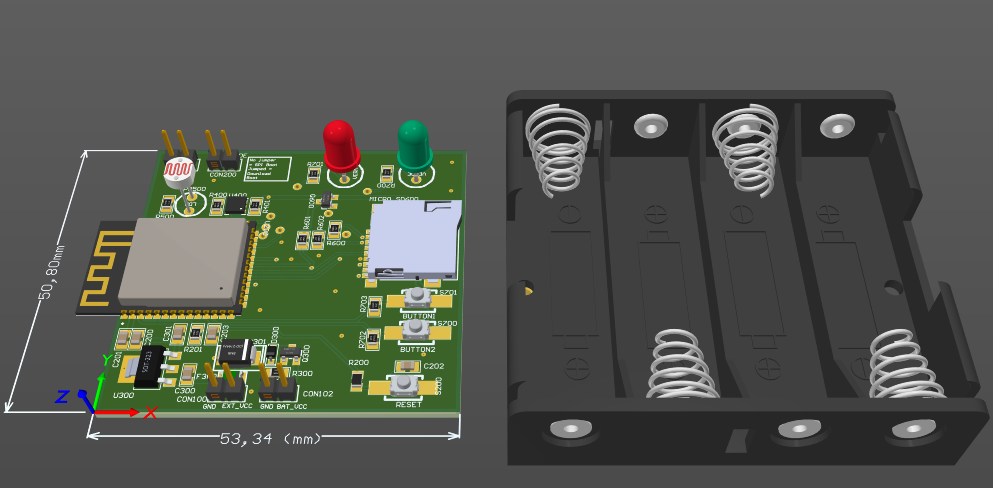
\includegraphics[width=\linewidth]{figuras/cap3/pcb/printd_3d_pcb.png}
				\source{Elaborado pelo autor.}
			\end{figure}

		\end{columns}


	}
	
\end{frame}


\begin{frame}{Produção}

	
	
	\only<1>{
		
		\framesubtitle{Materiais}
		\begin{itemize}
			\item Fornecedor de Componentes
			\begin{itemize}
				\item LCSC Electronics
			\end{itemize}
			\item Fabricação e Montagem PCI
			\begin{itemize}
				\item JLCPCB
			\end{itemize}

		\end{itemize}

		
		\begin{table}[!h]
			\captionsetup{width=9cm}%Deixe da mesma largura que a tabela
			\caption{\label{tab:custos_fabricacao} Custo de materiais por unidades}%
			% 	
			\begin{tabular}{cccc}
					\toprule
					Quantidade & Custo de Materiais  \\
					\midrule \midrule
					50 &  US\$ 502,60  \\
					100 &  US\$ 938,41 \\
					1000 & US\$ 8.736,80  \\
					\bottomrule
				\end{tabular}%
				% 	}
				\source{o autor.}%
			\end{table}    
			
			
			
		}


	\only<2>{

	
		\framesubtitle{Fabricação e Montagem}
		% \begin{itemize}
		% 	\item JLCPCB
		% 	\begin{itemize}
		% 		\item Fabricação PCI;
		% 		\item Montagem PCI.
		% 	\end{itemize}

			% \item 
		% \end{itemize}


		% \begin{columns}

			% \column{0.5\linewidth}
			\begin{table}[!h]
			\captionsetup{width=9cm}%Deixe da mesma largura que a tabela
			\caption{\label{tab:custos_montagem} Custos de Fabricação e Montagem}%
			\resizebox{0.6\textwidth}{!}{
				\begin{tabular}{cccc}
					\toprule
					Quantidade & Fabricação & Montagem & Total \\
					\midrule \midrule
					50 &  US\$ 22,4 & US\$ 64,47 & US\$ 86,87 \\
					100 &  US\$ 34,4 & US\$ 96,97 & US\$ 131,37 \\
					1000 & US\$ 249,70 & US\$ 447,92 & US\$ 667,62 \\
					\bottomrule
				\end{tabular}%
			}
			% \tiny{o autor.}%
			\source{o autor.}%
			\end{table}

			\vspace{-15pt}
			% \column{0.5\linewidth}
			\begin{table}[!h]
				\captionsetup{width=7cm}%Deixe da mesma largura que a tabela
				\caption{\label{tab:custos_fabricacao_unitario} Custo Unitário}%
				\resizebox{0.5\textwidth}{!}{
					\begin{tabular}{cccc}
						\toprule
						Quantidade & Custo Total & Custo Unitário  \\
						\midrule \midrule
						50 &  US\$ 582,42 & US\$ 11,65 \\
						100 &  US\$ 1048,93 & US\$ 10,49  \\
						1000 & US\$ 9261,29 & US\$ 9,26  \\
						\bottomrule
					\end{tabular}%
				}
					
				\source{o autor.}%
				
			\end{table}

		% \end{columns}





	}



    % \only<3>{


	% 	\framesubtitle{Custos unitários}



	% 	\begin{columns}
			
	% 		\column{0.5\linewidth}
	% 		\begin{table}[!h]
	% 			\captionsetup{width=7cm}%Deixe da mesma largura que a tabela
	% 			\caption{\label{tab:custos_fabricacao_unitario} Custo unitário}%
	% 			\resizebox{0.9\linewidth}{!}{
	% 				\begin{tabular}{cccc}
	% 					\toprule
	% 					Quantidade & Custo Total & Custo Unitário  \\
	% 					\midrule \midrule
	% 					50 &  US\$ 582,42 & US\$ 11,65 \\
	% 					100 &  US\$ 1048,93 & US\$ 10,49  \\
	% 					1000 & US\$ 9261,29 & US\$ 9,26  \\
	% 					\bottomrule
	% 				\end{tabular}%
	% 			}
					
	% 			\source{o autor.}%
				
	% 		\end{table}

	% 		\column{0.5\linewidth}

	% 			\begin{table}[!h]
	% 				\captionsetup{width=9cm}%Deixe da mesma largura que a tabela
	% 				\caption{\label{tab:custos_transporte} Custos de transporte para o Brasil}%
	% 				\resizebox{0.6\linewidth}{!}{
	% 						\begin{tabular}{cc}
	% 							\toprule
	% 							Quantidade & Valor  \\
	% 							\midrule \midrule
	% 							50 &  US\$ 80,36   \\
	% 							100 &  US\$ 110,52 \\
	% 							1000 & US\$ 524,49 \\
	% 							\bottomrule
	% 						\end{tabular}%
	% 				}
	% 				\source{o autor.}%
	% 			\end{table}


	% 	\end{columns}






	% }


\end{frame}
% \begin{frame}{Produção - custo frete}
% \end{frame}

\begin{frame}{Custos de Importação}




	Fatores considerados durante o cálculo dos custos de importação: 

	\begin{itemize}
		\item Cotação: R\$5,13 p/ cada Dólar;
		\item Imposto de importação zerado;
		\item ICMS para o estado do Ceará.
	\end{itemize}

	
	\begin{table}[!h]
	\captionsetup{width=10cm}%Deixe da mesma largura que a tabela
	\caption{\label{tab:custos_importacao} Custos de importação para o Brasil}
		\resizebox{0.5\linewidth}{!}{
		\begin{tabular}{ccccccccc}
			\toprule
			Quantidade & Valor & Frete & IPI & PIS & COFINS & ICMS & Total & Valor Unitário  \\
			\midrule \midrule
            50   & 2.576,22  & 412,35   & 38,85  & 62,76  & 288,40   & 741,64    & 4.120,22  & 82,40 \\
            100  & 4.815,26  & 567,11   & 69,97  & 113,03 & 519,40   & 1.335,68  & 7.420,46  & 74,20 \\
            1000 & 44.831,14 & 2.691,32 & 617,79 & 997,97 & 4.585,92 & 11.793,10 & 65.517,24 & 65,52\\
			\bottomrule
		\end{tabular}%
		}
		\source{o autor.}%

	\end{table}



    
\end{frame}

% \subsection{Energia}
\begin{frame}{Energia}

	\begin{table}[!h]
	\captionsetup{width=9cm}%Deixe da mesma largura que a tabela
	\caption{\label{tab:consumos_circuitos} Consumo por circuito em uso ativo}%
% 	
		\begin{tabular}{cc}
			\toprule
			Circuito & Consumo \\
			\midrule \midrule
			Controle  &  30  mA \\
			Sensores  &  27 mA  \\
			Circuito microSD   &   100 mA\\
			Interface de Usuário & 60 mA\\
		    \bottomrule
		\end{tabular}%
% 	}
	{%
	\tiny{o autor.}%
% 	\Nota{esta é uma nota, que diz que os dados são baseados na
% 		regressão linear.}%
% 	\Nota[Anotações]{uma anotação adicional, seguida de várias outras.}%
    }
    \end{table}

	\begin{table}[!h]
	\captionsetup{width=9cm}%Deixe da mesma largura que a tabela
	\caption{\label{tab:consumos_sono_profundo} Consumo por circuito em sono profundo}%
% 	
		\begin{tabular}{cc}
			\toprule
			Circuito & Consumo \\
			\midrule \midrule
			Controle  &  8 $\mu$A \\
			Sensores  &  0,2 $\mu$A  \\
			Regulador de tensão  & 65 $\mu$A\\
			Circuito microSD & 450$\mu$A \\
			Interface de Usuário & 0 $\mu$A \\
		    \bottomrule
		\end{tabular}%
% 	}
	{%
	\tiny{o autor.}%
% 	\Nota{esta é uma nota, que diz que os dados são baseados na
% 		regressão linear.}%
% 	\Nota[Anotações]{uma anotação adicional, seguida de várias outras.}%
    }
    \end{table}


    
\end{frame}


\begin{frame}{Comparativo de mercado}
    
    \begin{table}[!h]
    	
    	\captionsetup{width=9cm}%Deixe da mesma largura que a tabela
    	\caption{\label{tab:compara_dimensoes} \textit{Comparativo: Dimensões e Autonomia}}%
    % 	\resizebox{\textwidth}{!}{
    	
    		\begin{tabular}{cccc}
    			\toprule
    			Modelo & Dimensões & Nível de Proteção  & Autonomia \\
    			\midrule \midrule
               RCW-360           & Não informado   & IP64/IP65 & 3 meses       \\
               EL-WiFi-TH        & 82 x 70 x 23 mm & IP55  &6 meses       \\
               TandD RTR-507B    & 62 x 47 x 19 mm & IP64  &10 meses      \\
               160 TH            & 76 x 64 x 22 mm & IP20  & Não informado \\
               Hardware Proposto & 51 x 53 x 25 mm & Não possui & 2 meses  \\
    	    \bottomrule
    		\end{tabular}%
    % 	}{%
    	\tiny{o autor.}%

    \end{table}

    



    
\end{frame}





\begin{frame}{Comparativo - Precisão}


\begin{table}[!h]
	
	\captionsetup{width=9cm}%Deixe da mesma largura que a tabela
	\caption{\label{tab:compara_precisao} \textit{Comparativo: Faixa de leitura e Precisão}}%
% 	\resizebox{\textwidth}{!}{
	
		\begin{tabular}{ccccccc}
			\toprule
			Modelo & Faixa de Leitura (ºC) & Precisão (ºC) & Umidade Relativa (\%) & Precisão(\%)\\
			\midrule \midrule
           RCW-360           & -35 a 80      & 0,5 & 0 a 99 & 5    \\
           EL-WiFi-TH        & -20 a 60      & 0,3 & 0 a 100 & 2    \\
           TandD RTR-507B    & -25 a 70      & 0,3 & 0 a 99  & 2,50 \\
           160 TH            & -30 a 50      & 0,1 & 0 a 100 & 2 \\
           Hardware Proposto & -20 a 85      & 0,4 & 0 a 100 & 2\\
	    \bottomrule
		\end{tabular}%

	\tiny{o autor.}%

    \end{table}

    
\end{frame}





\begin{frame}{Comparativo - Preço Unitário}

    \begin{table}[!h]
	
	\captionsetup{width=7cm}%Deixe da mesma largura que a tabela
	\caption{\label{tab:compara_custo} \textit{Comparativo: Custo unitário}}%
% 	\resizebox{\textwidth}{!}{
	
		\begin{tabular}{cc}
			\toprule
			Modelo & Valor (R\$)\\
			\midrule \midrule
           RCW-360           & 1.499,00  \\
           EL-WiFi-TH        & 1.305,14  \\
           TandD RTR-507B    & 2.242,57 \\
           160 TH            & 2.842,00  \\
           Hardware Proposto & 65,52  \\
	    \bottomrule
		\end{tabular}%

	\tiny{o autor.}%

    % }
    \end{table}    
    
    
    \begin{table}[!h]
	
	\captionsetup{width=7cm}%Deixe da mesma largura que a tabela
	\caption{\label{tab:custos_extras} \textit{Comparativo: Custo unitário revisado}}%
% 	\resizebox{\textwidth}{!}{
	
		\begin{tabular}{cc}
			\toprule
			Modelo & Valor (R\$)\\
			\midrule \midrule
           RCW-360           & 1.499,00  \\
           EL-WiFi-TH        & 1.305,14  \\
           TandD RTR-507B    & 2.242,57 \\
           160 TH            & 2.842,00  \\
           Hardware Proposto & 142,35  \\
	    \bottomrule
		\end{tabular}%
	
	\tiny{o autor.}%

    \end{table}
    
\end{frame}

%% ---------------------------------------------------------------------------

% \begin{frame}{Criando Blocos}

% \end{frame}
